\section{Exercise 05: Drupal}


\subsection{Background}

\subsubsection{Which vulnerabilities do you think can be used? Pick two potential vulnerabilitiesand describe them in terms of why you picked them, i.e., date and exploit effect.}
For Exercise 5 on Drupal, I would focus on the drupal\_coder\_exec and drupal\_drupageddon vulnerabilities.
These vulnerabilities stand out due to their high exploitability rankings which for both of them are excellent.

The drupal\_drupageddon vulnerability presents a significant risk due to its nature as a SQL injection exploit.
Given that Drupal is a Content Management System (CMS), the potential impact of this exploit is substantial.
CMSs typically store user-generated content pages in databases that are rendered on websites.
Thus, a successful SQL injection attack could grant attackers access to extensive website data.
The severity of this vulnerability is reflected in its nickname, "drupageddon," indicating the widespread problems it caused when exploited.

Also the drupal\_coder\_exec vulnerability is particularly concerning because it stems from a third party plugin.
This aspect implies limited control by Drupal over the vulnerability, as opposed to an in-house developed component.
The critical nature of this exploit lies in its capability for arbitrary code execution,
offering a potent gateway for malicious actors to penetrate deeper into Drupal's server infrastructure.

Both vulnerabilities highlight critical security challenges in Drupal's system, especially considering their potential impacts and the nature of the weaknesses they exploit.


\subsubsection{For the rest of the tutorial, we will use the vulnerability dubbed \textit{drupageddon}. What is the underlying vulnerability?}
The underlying vulnerability is an SQL injection vulnerability.

\subsubsection{What is so severe about the issue?}
Drupal operates as a Content Management System (CMS), where website content is stored in databases.
Consequently, this setup permits a malicious actor to potentially access the entirety of these databases without proper authorization.


\subsection{Post-Exploitation}

\subsubsection{What are possible activities/aims for the post-exploitation phase?}
Having gained access to the machine, the first step is to secure the gotton access by establishing or compromising a user account.
This allows for continuous server access, enabling us to collect extensive information about the target system.
Additionally, we aim to elevate our privileges on the machine, further broadening our capability to acquire more detailed information.

\subsubsection{Write out the list in the file that has the “User Accounts”?}

\begin{tabular}{|l|l|l|l|}
    \hline
    root              & daemon        & bin               & sys          \\
    \hline
    sync              & games         & man               & lp           \\
    \hline
    mail              & news          & uucp              & proxy        \\
    \hline
    www-data          & backup        & list              & irc          \\
    \hline
    gnats             & nobody        & libuuid           & syslog       \\
    \hline
    messagebus        & sshd          & statd             & vagrant      \\
    \hline
    dirmngr           & leia\_organa  & luke\_skywalker   & han\_solo    \\
    \hline
    artoo\_detoo      & c\_three\_pio & ben\_kenobi       & darth\_vader \\
    \hline
    anakin\_skywalker & jarjar\_binks & lando\_calrissian & boba\_fett   \\
    \hline
    jabba\_hutt       & greedo        & chewbacca         & kylo\_ren    \\
    \hline
    mysql             & avahi         & colord            &              \\
    \hline
\end{tabular}


\subsubsection{How does having a list of user names help?}
Possessing a list of usernames makes the execution of brute force attacks easier by reducing the number of unknowns to guess.
Additionally, this list can be utilized in phishing campaigns, leveraging the available information to enhance the appearance of legitimacy.
In scenarios where users may have reused their usernames, and possibly passwords, across multiple sites,
checking against known password databases could reveal credentials that might grant access to the targeted website or system.


\subsubsection{What do the excellent post exploitation scripts for linux offer?}
The advanced post exploitation scripts for Linux provide a wealth of system information, including details on system versions, directories, and usernames.
Additionally, they offer capabilities for establishing persistent access through various backdoor mechanisms and other functionalities.


\subsection{Reflection}

\subsubsection{What is the main issue with the web server? How did it help selecting potentialexploits?}
The primary concern with the web server is its exposed directory listing.
This vulnerability not only enables the precise location of Drupal files to be visible but also gives access to Drupal via the drupal\_drupageddon exploit.
Such access highly aids in compromising the host machine.

\subsubsection{When opening the drupal web page, you are greeted by a warning. Do you think this is good practice? Why or why not?}

\begin{figure}[H]
    \centering
    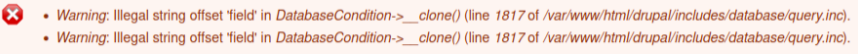
\includegraphics[width=0.9\linewidth]{pic/warning.png}
    \caption{warning}
    \label{fig:warning}
\end{figure}

Displaying a warning like this when going to the Drupal web page is not the best idea.
Such warnings could reveal details about the applications configuration, which could guiding an attacker to exploit existing security vulnerabilities.
Also, these warnings indicate possible misconfigurations in the Drupal server, which could suggest the presence of additional security weaknesses that might be exploited.
Its important for security to hide these messages from public view to prevent disclosing sensitive information.

\subsubsection{Given a more restrictive web server configuration, finding the relevant information wouldnt have been that easy. Please check dirbuster, to be found in the “Web Appli-cation Analysis” menu. How could this tool help you finding information? Try it outon the Ubuntu metasploitable VM. Use/ usr/ share/ dirbuster/ wordlists/ directory-list-2.3-medium.txtas dictionary.}

DirBuster is a tool designed to discover directories and files on a target server. By conducting a brute force attack, it will attempt various directory names,
sending multiple requests to uncover what directories exist on the server.

\begin{figure}[H]
    \centering
    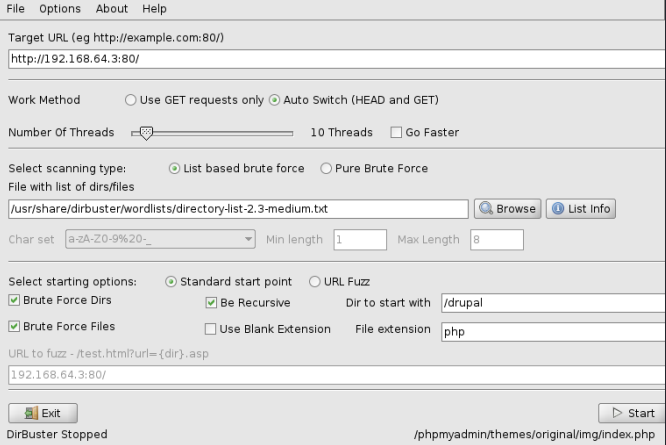
\includegraphics[width=0.9\linewidth]{pic/DirBuster App.png}
    \caption{DirBuster App}
    \label{fig:DirBuster App}
\end{figure}

This process results in a report detailing the servers directory structure.
For instance, to investigate the contents of a previously identified '/drupal' directory, DirBuster can be configured to focus its search within this specific path.
The outcome of such an operation provides insights into potential entry points and the overall structure of the server,
which is important for further penetration testing or security assessments.

\begin{figure}[H]
    \centering
    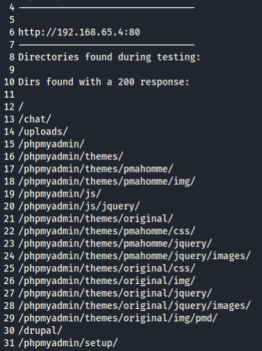
\includegraphics[width=0.4\linewidth]{pic/DirBuster.png}
    \caption{DirBuster}
    \label{fig:DirBuster}
\end{figure}


\subsubsection{How can effective spying with tools like dirbuster be prevented?}

To counteract the effectiveness of tools like DirBuster, several strategies can be employed

\begin{itemize}
    \item Avoid using predictable or common filenames, choose to do more randomized and obscure naming conventions to make brute force discovery less optimal.
    \item Employ rate limiting measures to restrict the number of requests a single user can make within a given timeframe, thereby counteracting the rapid request capability of DirBuster.
    \item Return a 404 status code for sensitive directories and files to give the impression that they do not exist, even if they do, thereby misleading automated scanning tools.
    \item Implement CAPTCHAs to challenge and filter out automated access attempts, making it difficult for tools like DirBuster to interact with the site without human intervention.
    \item Utilize firewalls to monitor and potentially block incoming traffic that exhibits patterns typical of directory brute-forcing tools.
    \item Set up robust monitoring systems with alerts to detect and respond to suspicious activities indicative of scanning attempts.
\end{itemize}
These methods contribute to a layered defense approach that can reduce the likelihood of successful spying by automated tools aimed at mapping server directories.


\subsubsection{This attack didnt get us all the way to root. How would you continue the pentest? What would be your next actions?}
The attack did not grant us root privileges, obtaining such access becomes easier once we have control over a
user with sudo capabilities. The logical next step is to use the sudo privileges to execute the \textit{sudo passwd root} command.
This would allow us to set a new password for the root user, which we could use to log in with full root access.
This would be the approach I would take to progress the penetration test.

\subsubsection{Do you have any specific things in mind you would try to get root access?}
When looking for the root access, I would consider exploiting the systems configuration by attempting to change the root password using the \textit{passwd} command.
Given the systems apparent misconfiguration, there is a chance that it might permit such an action, thereby granting me full control over the system.


\subsubsection{What makes getting a remote shell so powerful?}
Getting a remote shell is important due to the ability it grants an attacker to execute commands directly on a target machine.
This access can lead to the loose of high amounts of information. Essentially, the attacker can control the system and access most or all the data on the system,
thereby maximizing spying capabilities. Also, the remote nature of this access means that it can be conducted from anywhere, often without detection,
as many firewalls may not flag the shell's traffic, beliving its for legitimate outgoing connections.
